Based on the abstract system structure in presented in chapter \ref{chp:structure} a platform specific software structure needs to be defined for the Android OS platform.This structure is shown in figure \ref{android_structure}. It respects Android specific constructs, patterns and object-types.
\begin{figure}[h!]
\centering
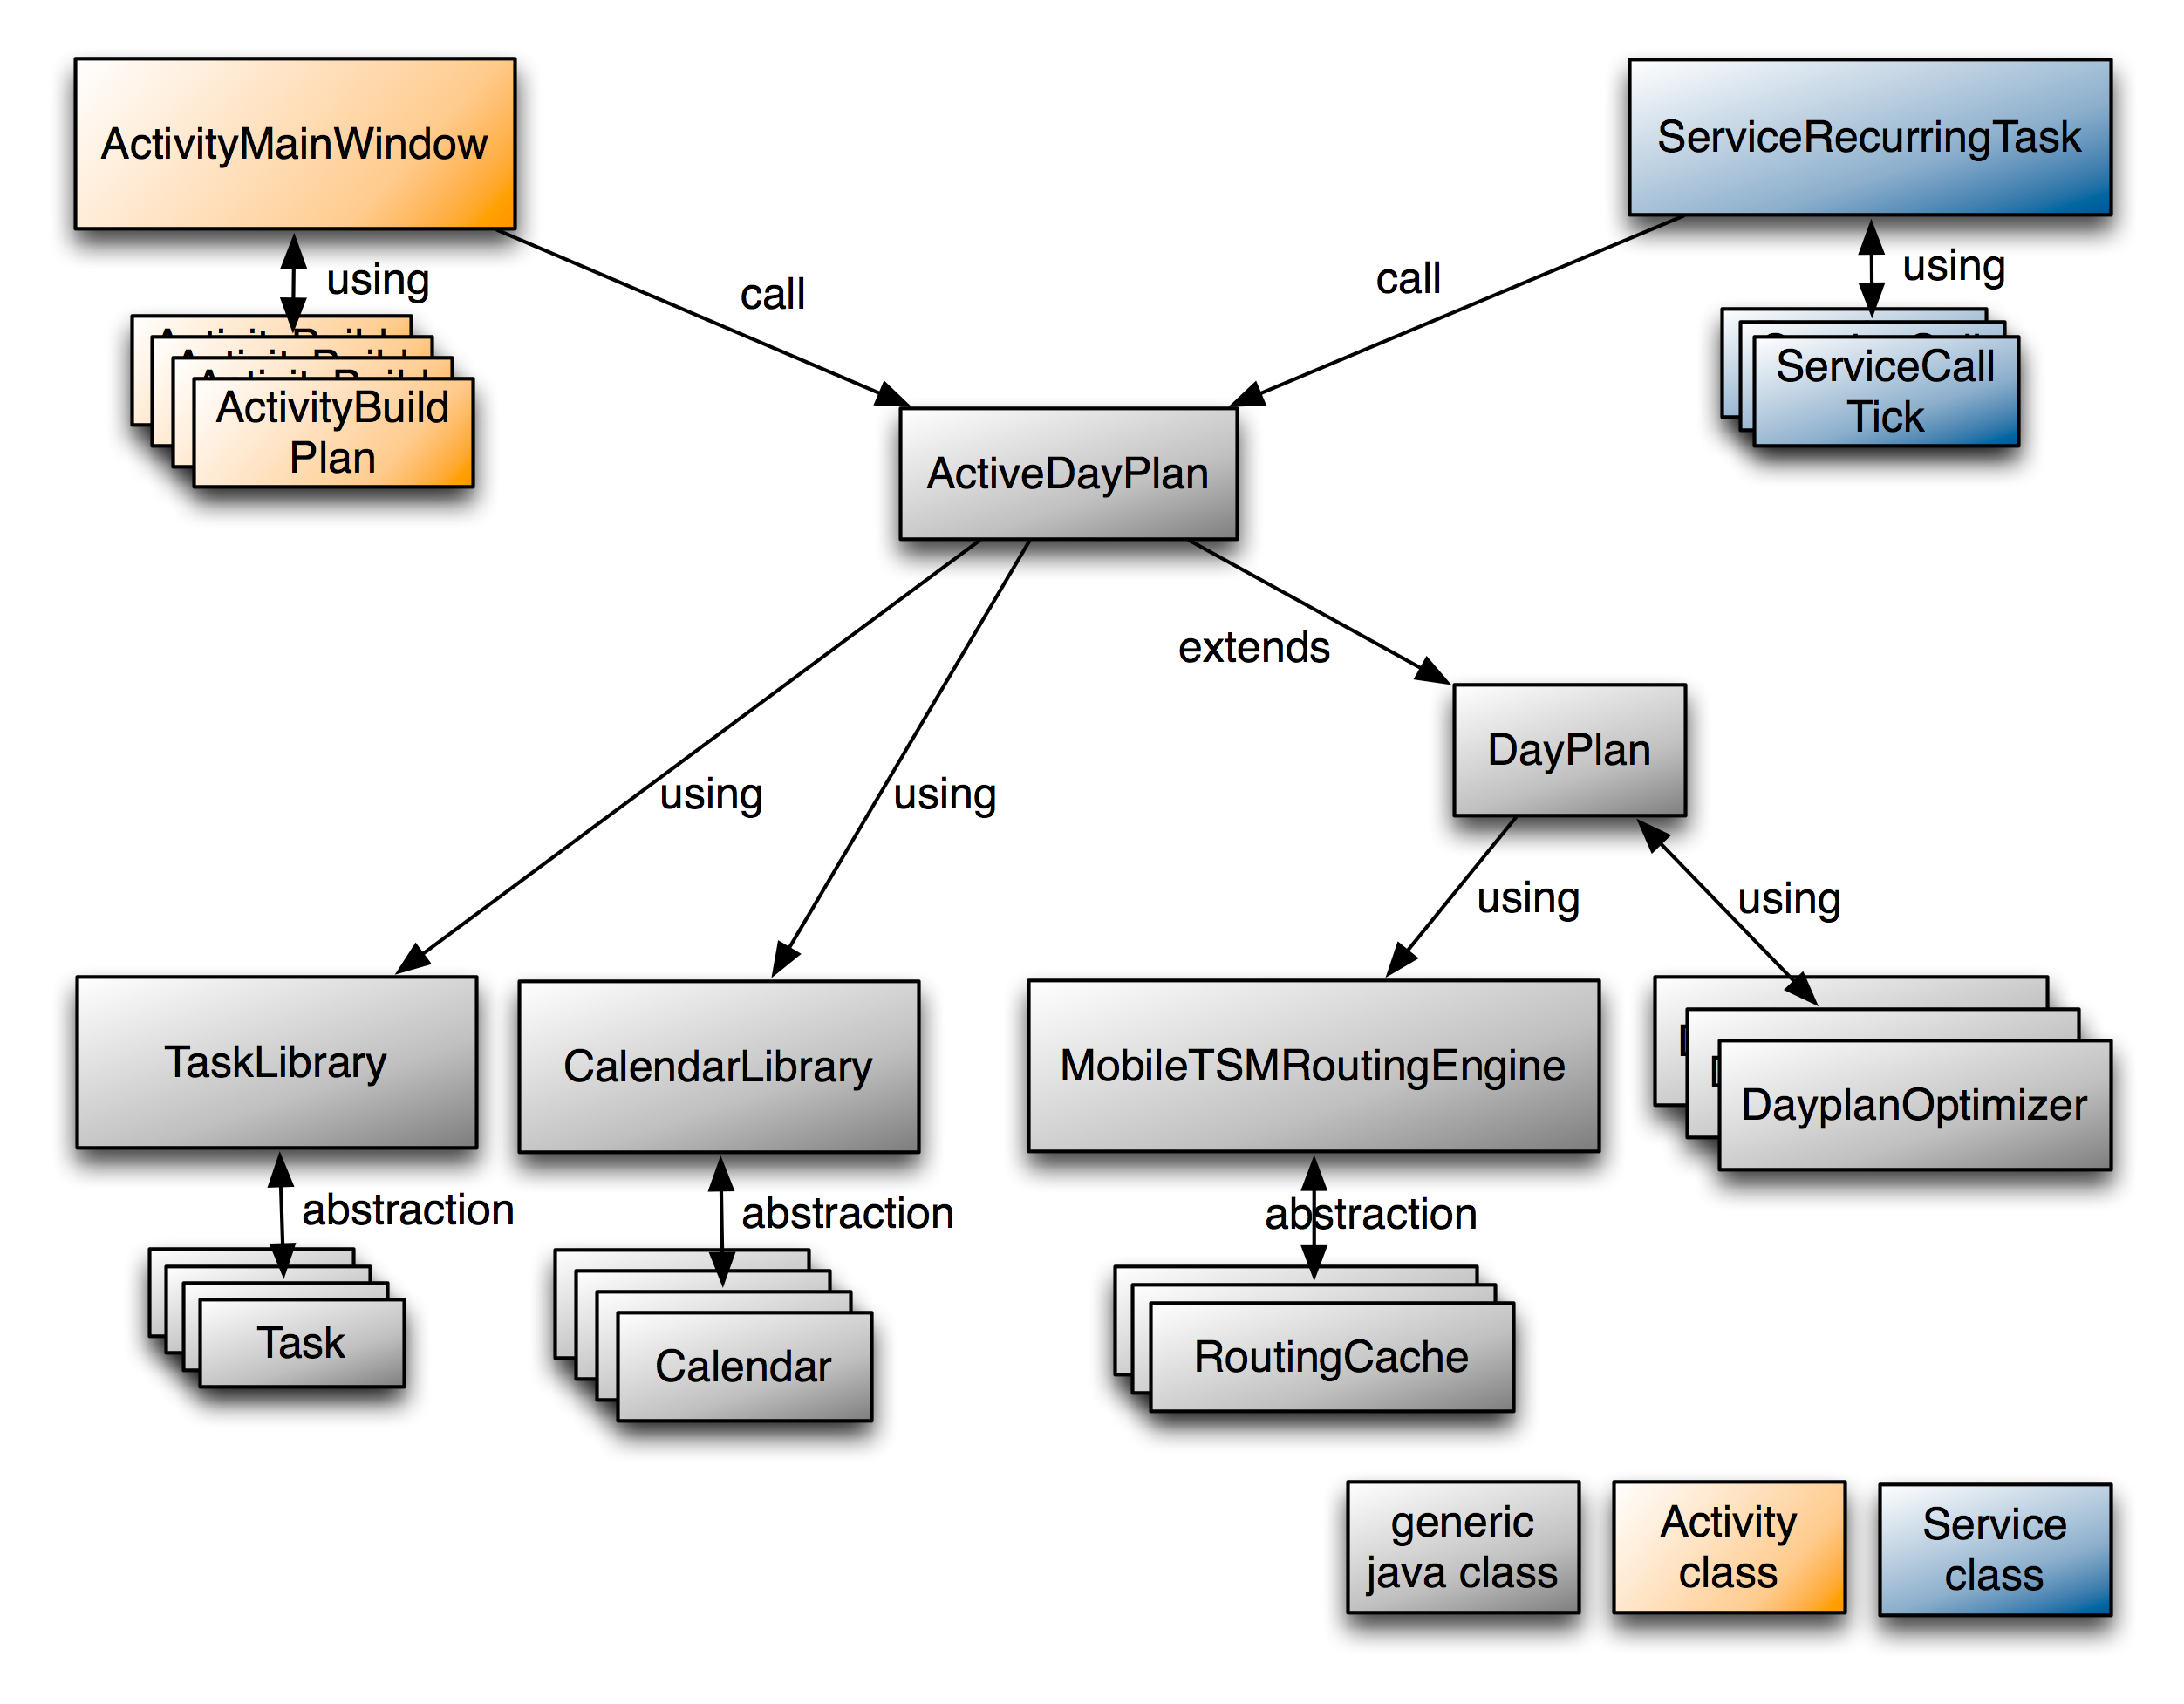
\includegraphics[width=14cm]{pics/android_structure.png}
\caption{Platform specific software structure for Android OS}
\label{android_structure}
\end{figure}
The classes marked in orange extend the platform specific Activity-class. In Android OS, Activities are used to build the graphical user interface (GUI). The class ActivityMainWindow contains a tabbing element, the other Activities are wrapped in the individual tabs. 

The blue classes extend the Service-class. Android OS uses Services to execute computations that are independent of the user interface. The background task that needs to be called cyclic is implemented in the ServiceRecurringTask. The other Services are helper classes that make sure the background task is called when the location of the device in time or space has changed.

All classes kept in grey are generic java classes. These system elements do not directly extend the Android platform, although some of them my use platform specific data types and methods.
  
TODO: describe the graphic\\
TODO: write why we did the design like that (briefly introduce android SW structure with services, activities etc.)